\section{Grundlagen}

\begin{defi}{Mikrocontroller}
    Ein \emph{Mikrocontroller} ist ein hochintegrierter Chip, der einen kompletten Rechner mit \emph{CPU}, \emph{Speicher} und diversen \emph{Schnittstellen} implementiert.

    In der Regel sind sie fest eingebettet in ein physikalisches System.

    Dabei verfolgen sie den Trend:
    \begin{itemize}
        \item immer kleiner,
        \item immer schneller,
        \item immer preiswerter,
        \item immer leistungsfähiger,
        \item immer weiter verbreitet
    \end{itemize}

    \vspace{1em}

    \begin{center}
        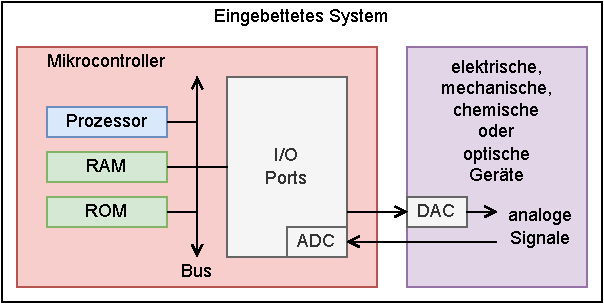
\includegraphics[width=0.75\textwidth]{includes/figures/defi_microcontroller.pdf}
    \end{center}
\end{defi}

\begin{bonus}{Unterschied Mikroprozessor und Mikrocontroller}
    Ein \emph{Mikroprozessor} nutzt externen Speicher.
    Dadurch es es möglich die Größe des Speichers beliebig zu wählen und im Betrieb auszutauschen.

    Ein \emph{Mikrocontroller} hat den gesamten Speicher intern eingebaut.
\end{bonus}

\begin{defi}{IoT}
    \emph{Internet of Things (IoT)} ist ein aktueller Technologietrend, bei dem extrem stromsparende Controller genutzt werden.

    Gegenständen des alltäglichen Lebens sollen immer stärker einbezogen und vernetzt werden.

    Dazu gehören z. B.:
    \begin{itemize}
        \item Autos
        \item Haushaltsgeräte
        \item Intelligente Sensoren
        \item medizinische Anwendungen
        \item Umweltschutz
        \item Kleidung
    \end{itemize}
\end{defi}

\begin{defi}{Eingebettetes System}
    Ein \emph{eingebettetes System} ist ein Computer, der in einen technischen Kontext eingebunden ist, bzw. Teil eines größeren Systems ist.
    Dabei übernimmt der Rechner entweder Überwachungs-, Steuerungs- oder Regelfunktionen oder ist für eine From der Daten- bzw. Signalverarbeitung zuständig.

    Eingebettete Software hat i. d. R. mit physikalischen Prozessen zu tun.
    Probleme dabei sind das Verwalten der Zeitanforderungen und ggf. auch der Nebenläufigkeit.

    Sie sind häufig reaktive Systeme\footnote{Klassische Systeme sind meist interaktive Systeme.}.
\end{defi}

\begin{bonus}{Moores Gesetz}
    \enquote{Alle 12-24 Monate verdoppelt sich die Anzahl der Transistoren auf einem Mikroprozessor, bzw. verdoppelt sich die Integrationsdichte.}

    Moores Gesetz lässt sich in abgeschwächter Form auch auf Mikrocontroller anwenden.
\end{bonus}

\begin{defi}{Technische Informatik}
    Wir befinden uns in der \emph{technischen Informatik}.
    Sie beschäftigt sich mit den hardwareseitigen und hardwarenahen Grundlagen der Informatik und ist unterteilt in:
    \begin{itemize}
        \item elektrotechnische und schaltungstechnische Grundlagen
        \item Rechnerstrukturen und -architekturen
        \item mathematische Grundlagen der Datenverarbeitung und Schaltungstechnik
        \item Dienstprogramme (Betriebssysteme, Linker, Lader etc.)
        \item Netzwerke, verteilte Systeme
    \end{itemize}

    Für das Verständnis sind elektronische Grundlagen der Informatik wichtig.
\end{defi}

\begin{defi}{ARM}
    \emph{Acorn Risc Machine (ARM)} ist eine seit den 80-Jahren existierende Prozessorarchitektur.
    ARM hat in den letzten Jahren verschiedene CPU-Architekturen entwickelt, die die Basis für unterschiedliche ARM-Prozessoren sind.

    Sie ist eine der ersten \emph{Reduced Instruction Set Computer (RISC)} Architekturen.

    Maschinensprache hat sich weiterentwickelt.
    Ursprünglich wurde ein \emph{32-Bit ARM}-Befehlssatz genutzt, heute verwendet man eher einen \emph{16-Bit Thumb} oder gemischten \emph{16/32-Bit Thumb2} Befehlssatz.
    Die Registrierungsstruktur aller Prozessoren ist weitgehend identisch.

    ARM verkauft keine fertigen Chips, sondern entweder die HW/SW-Spezifikationen für einen Prozessor oder das Recht, auf Basis der ARM-Architektur eigene ARM-kompatible Prozessoren zu entwickeln.
\end{defi}

\begin{bonus}{RISC vs. CISC}
    \begin{tabularx}{\textwidth}{|X|X|}
        \hline
        CISC                                               & RISC                                          \\\hline\hline
        Betonung der Hardware                              & Betonung der Software                         \\\hline
        Mehrere Befehlsgrößen und -formate                 & Befehle desselben Satzes mit wenigen Formaten \\\hline
        Weniger Register                                   & Verwendung von mehr Registern                 \\\hline
        Mehr Adressierungsmodi                             & Weniger Adressierungsmodi                     \\\hline
        Umfangreiche Verwendung von Mikroprogrammierung    & Komplexität im Compiler                       \\\hline
        Befehle benötigen eine unterschiedliche Zykluszeit & Anweisungen benötigen eine Zykluszeit         \\\hline
        Pipelining ist schwierig                           & Pipelining ist einfach                        \\\hline
    \end{tabularx}
\end{bonus}

\begin{defi}{Register des ARM Cortex M4 Prozessors}
    \begin{itemize}
        \item General purpose registers (32 bit): \texttt{R0} - \texttt{R12}
        \item Stack pointer: \texttt{R13 (MSP)} / \texttt{R13 (PSP)}
        \item Link register: \texttt{R14 (LR)}
        \item Program counter: \texttt{R15 (PC)}
    \end{itemize}

    \emph{Special registers}:
    \begin{itemize}
        \item \texttt{PSR} Program status Register
        \item \texttt{PRIMASK}
        \item \texttt{FAULTMASK}
        \item \texttt{BASEPRI}
        \item \texttt{CONTROL}
    \end{itemize}
\end{defi}

\begin{defi}{GPIO}
    \emph{General Purpose Input Output (GPIOs)} sind die einfachste Form binärer Signale (\texttt{HIGH}/\texttt{LOW})\footnote{\texttt{LOW} bedeutet idealerweise 0V; \texttt{HIGH} bedeutet idealerweise 3.3V} über einzelne Leitungen auszugeben.

    Die einzelnen Leitungen sind i. d. R. Ports mit jeweils acht Leitungen zusammengefasst;

    z. B. bedeutet \texttt{P4.3}: Port 4 Leitung 3.

    Jede einzelne Leitung kann als Ein- oder Ausgabe programmiert werden.
    Nach einem Reset sind alle GPIOs auf Eingabe gestellt.
\end{defi}

\begin{bonus}{Pullup bzw. Pulldown}
    Ein \emph{Pullup} bzw. \emph{Pulldown}-Widerstand dient dazu, den Zustand einer GPIO-Leitung auf einen definierten Wert zu legen, wenn die Leitung mit nichts verbunden ist.

    Sie können extern existieren oder im Mikrocontroller eingeschaltet werden.
\end{bonus}